%%%%%%%%%%%%%%%%%%%%%%%%%%%%%%%%%%%%%%%%%%%%%%%%%%%%%%%%%%%%%%%%%%%%DDATA TASK REPORT
%%%%%%%%%%%%%%%%%%%%%%%%%%%%%%%%%%%%%%%%%%%%%%%%%%%%%%%%%%%%%%%%%%%%%






\documentclass[12pt]{report}

\usepackage[a4paper]{geometry}
\usepackage[myheadings]{fullpage}
\usepackage{float}
\usepackage{fancyhdr}
\usepackage{amsmath}
\usepackage{adjustbox}
\usepackage{amsmath,upgreek,bm}
\usepackage{physics}
\usepackage{lastpage}
\usepackage{graphicx, wrapfig, subcaption, setspace, booktabs}
\newcommand{\citeColored}[2]{{\hypersetup{citecolor=#1}\cite{#2}}}
\usepackage{hyperref}
\usepackage[T1]{fontenc}
\usepackage[font=small, labelfont=bf]{caption}
\usepackage{fourier}
\usepackage[protrusion=true, expansion=true]{microtype}
\usepackage[english]{babel}
\usepackage{sectsty}
\usepackage{url, lipsum}
\usepackage{tgbonum}
\usepackage{hyperref}
\usepackage{xcolor}
\usepackage{threeparttable}
\usepackage[utf8]{inputenc}
\newcommand{\HRule}[1]{\rule{\linewidth}{#1}}
\onehalfspacing
\setcounter{tocdepth}{5}
\setcounter{secnumdepth}{5}
\usepackage{enumitem}
\usepackage{longtable}
\usepackage{rotating}
\usepackage{amsmath}
\DeclareRobustCommand{\bbone}{\text{\usefont{U}{bbold}{m}{n}1}}
\DeclareMathOperator{\EX}{\mathbb{E}}% expected value

\usepackage{graphicx}

\usepackage{xspace} 
\usepackage{multirow}
\usepackage{amsmath,amssymb}
\DeclareRobustCommand{\bbone}{\text{\usefont{U}{bbold}{m}{n}1}}
\usepackage{blindtext}
%\usepackage[flushleft]{threeparttable}
%\usepackage{booktabs, caption, makecell}
%\usepackage{chngcntr}
%\counterwithin{table}{section}
%-------------------------------------------------------------------------------
% TITLE PAGE : 
%-------------------------------------------------------------------------------
\begin{document}
{\fontfamily{cmr}\selectfont
\title{ \normalsize \textsc{}
		\\ [2cm]
		\HRule{0.5pt} \\
		\LARGE \textbf{\uppercase{Fertility and Education Patterns Across Different Phases of Development}
		\HRule{2pt} \\ [0.5cm]
		\normalsize  \vspace*{5\baselineskip}}
		}

\date{September 2nd, 2020}

\author{
		Alexander Quispe Rojas \\ 
		}

\maketitle
\tableofcontents
\newpage

%-------------------------------------------------------------------------------
% Section title formatting
\sectionfont{\scshape}
%-------------------------------------------------------------------------------

%-------------------------------------------------------------------------------
% BODY
%-------------------------------------------------------------------------------

\section{Theoretical Model}

Ohinata \& Varvarigos (2020) propose a model where the economy is populated by overlapping generations of households that have
a lifespan of two periods: childhood and adulthood. The household’s budget constraint is

    \begin{equation}
    \begin{aligned}
    c_{t} = \omega h_{t} - n_{t}(q+x_{t})
    \end{aligned}
    \end{equation}

where $c_{t}$ denotes consumption and $h_{t}$ is the stock of human capital.Besides, $\omega$ is the wage per unit of effective labour, and  rearing each child entails a fixed cost of $q>0$. Parents spend resources towards the education of each of their offspring using $x_t$ amount.  

Parents can affect each child’s human capital by devoting resources towards their education using $x_t$ units, so the human capital will be determined as : 

    \begin{equation}
    \begin{aligned}
    h_{t+1} = \varphi h_{t}^{\eta} + \psi h_{t}^{\mu}x_t 
    \end{aligned}
    \end{equation}

Where $\phi , \psi > 0$ and $\eta , \mu  \in (0, 1)$. Note that $h_t$ captures intergenerational externalities that generate dynamics in the formation of human capital. The lifetime utility of the household is given by:

    \begin{equation}
    \begin{aligned}
    u_{t} = \gamma \ln(c_t) + (1-\gamma)[\beta \ln(n_t) + \theta \ln(n_t h_{t+1})]
    \end{aligned}
    \end{equation}
    
Households make their choices so as to maximize their lifetime utility in
equation (3), subject to the constraints in equations (1) and (2). The first order condition are :

    \begin{equation}
    \begin{aligned}
    n_t (q+x_t) = \frac{(1-\gamma)(\beta + \theta)}{\gamma + (1-\gamma)(\beta + \theta)} \omega h_t \\
    x_t = \frac{(1-\gamma)\theta}{\gamma + (1-\gamma)(\beta + \theta)}\frac{\omega h_t}{n_t} - \frac{\varphi}{\psi} h_t^{\eta - \mu}
    \end{aligned}
    \end{equation}

The system of equations in (4) can be solved simultaneously to

    \begin{equation}
    \begin{aligned}
    x_t = X(h_t)  = \max \{0, \frac{1}{\beta}[\theta q - (\theta + \beta) \frac{\varphi}{\psi}  h_t^{\eta - \mu}]\}
    \end{aligned}
    \end{equation}
    
and

    \begin{equation}
    \begin{aligned}
    n_t = N(h_t)  = \begin{cases}
                    \frac{(1-\gamma)(\beta + \theta)}{\gamma + (1-\gamma)(\beta + \theta)} \frac{\omega h_t}{q} & \text{if } x_t = 0 \\
                    \frac{(1-\gamma)\beta}{\gamma + (1-\gamma)(\beta + \theta)} \frac{\omega \psi h_t^{1 + \mu - \eta }}{q \psi h_t^{\mu - \eta} - \varphi}   & \text{if } x_t > 0
                     \end{cases}
    \end{aligned}
    \end{equation}
    
A closer look at the result in equation (5) reveals that there are circumstances under which parents might find it optimal not to invest any
resources towards the education of their offspring.The underlying cause for this possibility lies in the fact that, as long as $ \varphi > 0$, each child will still be endowed with units of efficient labour, because of the presence of the intergenerational externality, even though parents might not invest any resources towards their education.\\

\subsection{Dynamics} 

Assumming that  $\mu > \eta $ , when the stock of human capital is relatively low, the utility cost of foregone consumption outweighs the utility
benefit of educating children and increasing their efficiency. Nevertheless, when the stock of human capital is relatively high, its complementary
effect becomes strong enough to guarantee that the return to investment in education is sufficiently high to compensate parents for the utility loss
due to decreased consumption.

\textbf{Lemma 1}: There exist a threshold which comes when the second element of $X$ functions is equalized to zero : 

    \begin{equation}
    \begin{aligned}
    \Tilde{h} \equiv \left[\frac{(\theta + \beta)\varphi}{\theta \psi q}\right]^{\frac{1}{\mu - \eta}}
    \end{aligned}
    \end{equation}

such that 
    \begin{equation}
    \begin{aligned}
    x_t = X(h_t)  = \begin{cases}
                    0 & \text{if } h_t <= \Tilde{h} \\
                     \frac{1}{\beta}\left[\theta q - (\theta + \beta) \frac{\varphi}{\psi}  h_t^{\eta - \mu}\right] & \text{if } h_t > \Tilde{h}
                     \end{cases}
    \end{aligned}
    \end{equation}

We can see that $ X(\Tilde{h}) = 0$ and 

    \begin{equation}
    \begin{aligned}
    X'(h_t) = \frac{(\mu - \eta)(\theta + \beta)\varphi}{\beta\psi}h_{t}^{\eta - \mu-1} > 0
    \end{aligned}
    \end{equation}

The outcome summarized in (7) allows us to combine equations in order to express human capital accumulation as : 
    \begin{equation}
    \begin{aligned}
    h_{t+1} = F(h_t)  = \begin{cases}
                    \varphi h_{t}^{\eta}  & \text{if } h_t <= \Tilde{h} \\
                     \frac{\theta (\psi q h_{t}^{\mu} - \varphi h_{t}^{\eta})}{\beta}  & \text{if } h_t > \Tilde{h}
                     \end{cases}
    \end{aligned}
    \end{equation}

Fertility Dynamics:
We begin the analysis by using the results in equation (6) in order to examine how fertility varies with the stock of human capital.
\textbf{Lemma 2} :
Consider $n_t = N(h_t)$. It is straightforward to establish that (a) when $x_t = 0$ then $N(h_t)>0$ ; (b) when $x_t > 0$ then there exists. 
   
    \begin{equation}
    \begin{aligned}
    \hat{h} \equiv \left[\frac{(1+\mu - \eta)\varphi}{\psi q}\right]^{\frac{1}{\mu - \eta}}
    \end{aligned}
    \end{equation}

such that when $x_t = 0$
    \begin{equation}
    \begin{aligned}
        N'(h_t) = \frac{(1-\gamma)(\beta +  \theta)}{\gamma + (1-\gamma)(\beta + \theta)}\frac{\omega}{q} > 0 
    \end{aligned}
    \end{equation}

but when $x_t > 0$
    \begin{equation}
    \begin{aligned}
        N'(h_t) & = \frac{(1-\gamma)(\beta)}{\gamma + (1-\gamma)(\beta + \theta)q}\omega\psi \\
        & X\left[\frac{(1+\mu + \eta)h_{t}^{\mu - \eta} (q \psi h_{t}^{\mu - \eta} - \varphi) - h_{t}^{1+\mu - \eta}(\mu - \eta)(q \psi h_{t}^{\mu - \eta -1})}{(q \psi h_{t}^{\mu - \eta} - \varphi)^{2}} \right]
    \end{aligned}
    \end{equation}

The sign of the derivative will depend on the sign of the expression inside the square brackets. 

    \begin{equation}
    \begin{aligned}
    N'(h_t) = \begin{cases}
                    < 0     & \text{if } h_t <= \hat{h} \\
                    > 0     & \text{if } h_t > \hat{h}
                     \end{cases}
    \end{aligned}
    \end{equation}

\textbf{Lemma 3}: 
As long as $[(1+\mu - \eta )\theta]/(\theta + \beta)>1$ then $\hat{h} > \Tilde{h}$
Prrof: $\hat{h} > \Tilde{h}$ implies

    \begin{equation}
    \begin{aligned}
    \left[\frac{(1+\mu - \eta)\varphi}{\psi q}\right]^{\frac{1}{\mu - \eta}} >  \left[\frac{(\theta + \beta)\varphi}{\theta \psi q}\right]^{\frac{1}{\mu - \eta}}
    \end{aligned}
    \end{equation}

And this is only true if  $[(1+\mu - \eta )\theta]/(\theta + \beta)>1$ then $\hat{h} > \Tilde{h}$. \\

Therefore, as the stock of human capital grows, the fertility rate increases for $h_t < \tilde{h}$; it declines for $\Tilde{h} < h_t < \hat{h}$; and it increases again for $h_t > \hat{h}$.
Formally,

    \begin{equation}
    \begin{aligned}
    N'(h_t) = \begin{cases}
                    > 0     & \text{if } h_t < \Tilde{h} \\
                    < 0     & \text{if } \Tilde{h} < h_t <= \hat{h} \\
                    > 0     & \text{if } h_t > \hat{h} \\
                    \end{cases}
    \end{aligned}
    \end{equation}
    
Specifically, the fertility rate increases with $h_t$ at relatively low levels of income; it decreases at intermediate levels of income; and it increases again at relatively high levels of income, as the stock of human capital and therefore fertility converge to their long-run (steady-state) values.

Naturally, our objective is to analyse an economy that goes through all the stages of possible demographic changes, as it converges to the longrun equilibrium that is characterized by $h^{*}$.It follows that the subsequent
analysis will focus on a scenario where the steady-state equilibrium lies
above the two thresholds identified previously. \\
\textbf{Lemma 4}: Assume that.

    \begin{equation}
    \begin{aligned}
    q\psi > max \left\{ \left(\frac{\beta}{\theta}\right)^{(\mu - \eta)/(1-\eta)} \frac{(1+\mu -\eta)\varphi^{(1-\mu)/(1-\eta)}}{(\mu - \eta)^{(\mu - \eta)/(1-\eta)}};\frac{(\theta + \beta) \varphi^{(1-\mu)/(1-\eta)}}{\theta} \right\}
    \end{aligned}
    \end{equation}
    
holds. Then $h^{*} > \hat{h}$ \\

\subsection{The full dynamical system} 
The full dynamics of this model are characterized by a non-linear three dimensional system of difference equations.
        \begin{equation}
    \begin{aligned}
    h_{t+1} = F(h_t)  &= \begin{cases}
                    \varphi h_{t}^{\eta}  & \text{if } h_t <= \Tilde{h} \\
                     \frac{\theta (\psi q h_{t}^{\mu} - \varphi h_{t}^{\eta})}{\beta}  & \text{if } h_t > \Tilde{h}
                     \end{cases}\\
    x_t = X(h_t)  &= \max \{0, \frac{1}{\beta}[\theta q - (\theta + \beta) \frac{\varphi}{\psi}  h_t^{\eta - \mu}]\} \\
    n_t = N(h_t)  &= \begin{cases}
                \frac{(1-\gamma)(\beta + \theta)}{\gamma + (1-\gamma)(\beta + \theta)} \frac{\omega h_t}{q} & \text{if } x_t = 0 \\
                \frac{(1-\gamma)\beta}{\gamma + (1-\gamma)(\beta + \theta)} \frac{\omega \psi h_t^{1 + \mu - \eta }}{q \psi h_t^{\mu - \eta} - \varphi}   & \text{if } x_t > 0
                 \end{cases}
    \end{aligned}
    \end{equation}

This line is added to see if overleaf and github fits well. 


%\newpage
%\section{Getting Started}
%\input{getstart.tex}

% \section{Question 2}
% %\begin{enumerate}[label=(\alph*)]


Consider the constant elasticity of substitution (CES) production function

    \begin{equation}
    \begin{aligned}
    F(K,L) = (\alpha K^{\rho} + (1-\alpha)L^{\rho})^{1/\rho}
    \end{aligned}
    \end{equation}
with $\rho \in (-\infty,1]$ and $ \alpha \in (0,1)$.

\begin{itemize}
\item 
CES is CRTS

    \begin{equation}
    \begin{aligned}
    F(\lambda K,\lambda L) = (\alpha (\lambda K)^{\rho} + (1-\alpha)(\lambda L)^{\rho})^{1/\rho} \\
    F(\lambda K,\lambda L) = (\lambda^{\rho}(\alpha (K)^{\rho} + (1-\alpha)(L)^{\rho}))^{1/\rho} \\
    F(\lambda K,\lambda L) = \lambda(\alpha (K)^{\rho} + (1-\alpha)(L)^{\rho})^{1/\rho} 
    \end{aligned}
    \end{equation}

\item 
Derive conditional factor demands $(K^{c},L^{c})$ and the CES cost function.
From FOC we have ,

    \begin{equation}
    \begin{aligned}
        & F_{L} = \frac{1}{\rho}(\alpha K^{\rho} + (1-\alpha)L^{\rho})^{(1/\rho)-1}[(1-\alpha) \rho L^{\rho-1}] = w \\
        & F_{K} = \frac{1}{\rho}(\alpha K^{\rho} + (1-\alpha)L^{\rho})^{(1/\rho)-1}[\alpha \rho K^{\rho-1}] = r \\
        & \frac{F_{L}}{F_{K}} = \frac{(1-\alpha)L^{\rho-1}}{(\alpha)K^{\rho-1}}=\frac{w}{r} \\
        & K = (\frac{\alpha}{1-\alpha}\frac{w}{r})^{\frac{1}{1-\rho}}L  ;\  
        L = (\frac{r}{\alpha})^{\frac{-1}{\rho-1}}
        (\frac{w}{1-\alpha})^{\frac{1}{\rho-1}}K
    \end{aligned}
    \end{equation}

So we need to plug the last equation in the Production function for a level $F(K,L)=\bar{q}$.

    \begin{equation}
    \begin{aligned}
    F(K,L) =\bar{q} =(\alpha K^{\rho} + (1-\alpha)[(\frac{r}{\alpha})^{\frac{-1}{\rho-1}}
        (\frac{w}{1-\alpha})^{\frac{1}{\rho-1}}K]^{\rho})^{1/\rho}
    \end{aligned}
    \end{equation}

with this equation we can find the conditional demand of capital and then using the optimal condition in (7) to find the Labor demand. 

    \begin{equation}
    \begin{aligned}
    K^{c}=\frac{\bar{q}(\frac{r}{\alpha})^{\frac{1}{\rho-1}}}
        {[\alpha(\frac{r}{\alpha})^{\frac{\rho}{\rho-1}}+
        (1-\alpha)(\frac{w}{1-\alpha})^{\frac{\rho}{\rho-1}}]^{\frac{1}{\rho}}} \\
    L^{c} =\frac{\bar{q}(\frac{w}{1-\alpha})^{\frac{1}{\rho-1}}}
        {[\alpha(\frac{r}{\alpha})^{\frac{\rho}{\rho-1}}+
        (1-\alpha)(\frac{w}{1-\alpha})^{\frac{\rho}{\rho-1}}]^{\frac{1}{\rho}}} 
    \end{aligned}
    \end{equation}

then we can find the CES cost function

    \begin{equation}
    \begin{aligned}
    C(\bar{q}) = r\frac{\bar{q}(\frac{r}{\alpha})^{\frac{1}{\rho-1}}}
        {[\alpha(\frac{r}{\alpha})^{\frac{\rho}{\rho-1}}+
        (1-\alpha)(\frac{w}{1-\alpha})^{\frac{\rho}{\rho-1}}]^{\frac{1}{\rho}}} +
    w\frac{\bar{q}(\frac{w}{1-\alpha})^{\frac{1}{\rho-1}}}
        {[\alpha(\frac{r}{\alpha})^{\frac{\rho}{\rho-1}}+
        (1-\alpha)(\frac{w}{1-\alpha})^{\frac{\rho}{\rho-1}}]^{\frac{1}{\rho}}} 
    \end{aligned}
    \end{equation}

\item 
The elasticity of technical substitution for CES production.

    \begin{equation}
    \begin{aligned}
    \sigma = \frac{d\ln{K/L}}{d\ln{w/r}} =
    \frac{d\ln{(\frac{\alpha}{1-\alpha}\frac{w}{r})^{\frac{1}{1-\rho}}}}{d\ln{w/r}}=
    \frac{\frac{1}{1-\rho}
    d[{ \ln{\frac{w}{r}} + \ln{\frac{\alpha}{1-\alpha}}]
    }}{d\ln{w/r}}= \frac{1}{1-\rho}
    \end{aligned}
    \end{equation}

\item 
CES function might become into different functions depending on the values of $\rho$.
When $\rho = 1$ then we have the linear function. 

    \begin{equation}
    \begin{aligned}
    F(K,L) = \alpha K + (1-\alpha)L
    \end{aligned}
    \end{equation}

When $\rho = 0$ then we get the Cobb–Douglas production function. To prove this first we need to take ln of F(K,L) ,

    \begin{equation}
    \begin{aligned}
    \ln{F(K,L)} = \frac{1}{\rho} \ln((\alpha k^{\rho} + (1-\alpha)L^{\rho}))
    \end{aligned}
    \end{equation}

We need to use l'Hôpital's rule to show the convergence to the Cobb-Douglas function when $\lim_{\rho\to 0}\ln{F(K,L)}$ and we can use the continuity properties from the production function. 

    \begin{equation}
    \begin{aligned}
        \lim_{\rho\to 0}\ln{F(K,L)} 
        & = \lim_{\rho\to 0} \frac{\frac{1}{\alpha k^{\rho} + (1-\alpha)L^{\rho}}
        [\alpha k^{\rho}\ln{K} + (1-\alpha)L^{\rho}\ln{L}]}{1} \\
        & = \alpha \ln{K} + (1-\alpha) \ln{L} \\
        &  =  \ln(K^{\alpha}L^{(1-\alpha)}) \Longrightarrow {F(K,L)} = K^{\alpha}L^{(1-\alpha)}
    \end{aligned}
    \end{equation}

When $\lim_{\rho \to -\infty}$ then we get the $\min{(K, L)}$ production function.
This exercise is similar to do $\lim_{\rho \to \infty}F(K,L,-\rho)$ where 

    \begin{equation}
    \begin{aligned}
    F(K,L,-p) = \frac{1}{(\alpha \frac{1}{K^{\rho}} + (1-\alpha)\frac{1}{L^{\rho}})^{1/\rho}}
    \end{aligned}
    \end{equation}

Let´s propose the next function 
    \begin{equation}
    \begin{aligned}
    U(K,L) = (\alpha \frac{1}{K^{\rho}} + (1-\alpha)\frac{1}{L^{\rho}})^{1/\rho}
    \end{aligned}
    \end{equation}

If we assume that $L<K \implies \frac{\alpha}{L^{\rho}} > \frac{\alpha}{K^{\rho}}$ and  $\frac{1-\alpha}{L^{\rho}} \geq  \frac{1-\alpha}{L^{\rho}} \implies 
\frac{1}{L^{\rho}} \geq  \frac{\alpha}{K^{\rho}} + \frac{1-\alpha}{L^{\rho}}$. \\
Therefore we conclude that the upper bound of U(K,L) is 

    \begin{equation}
    \begin{aligned}
    U(K,L) = (\alpha \frac{1}{K^{\rho}} + (1-\alpha)\frac{1}{L^{\rho}})^{1/\rho} \leq\frac{1}{L} 
    \end{aligned}
    \end{equation}

But is also true that 
    \begin{equation}
    \begin{aligned}
    (1-\alpha)^{\frac{1}{\rho}}\frac{1}{L} \leq U(K,L) = (\alpha \frac{1}{K^{\rho}} + (1-\alpha)\frac{1}{L^{\rho}})^{1/\rho} \leq\frac{1}{L} 
    \end{aligned}
    \end{equation}

Since we know that $F(K,L,-p) = [U(K,L)]^{-1}$ this implies that 
    \begin{equation}
    \begin{aligned}
     L \leq 
    F(K,L,-p) = \frac{1}{(\alpha \frac{1}{K^{\rho}} + (1-\alpha)\frac{1}{L^{\rho}})^{1/\rho}} \leq
    \frac{L}{(1-\alpha)^{\frac{1}{\rho}}}
    \end{aligned}
    \end{equation}

Then when we take the  $\lim_{\rho \to \infty}\frac{L}{(1-\alpha)^{\frac{1}{\rho}}}=L$ which sandwiches the middle term in (19) to L. Therefore we have proved that $\lim_{\rho \to -\infty}F(K,L,\rho) = \min{(K, L)}$.




\end{itemize}





%\end{enumerate}

%\section{Question 1}
%
Construct a PSID extract similar to the one used by Angrist (1991). PSID data are available
from the ISR:

\href{https://simba.isr.umich.edu/Zips/ZipMain.aspx}{https://simba.isr.umich.edu/Zips/ZipMain.aspx}

(use the cross-year index to select variables from family files).
\begin{enumerate}
    \item Calculate the grouped-data, Analysis of Covariance (fixed-effects), and OLS estimates of MaCurdy's (1981) specification reported by Angrist (1991, Table 3).
    \item
     How does Angrist (1991) explain differences in results across methods?
    \item
    Why does Card (1994) take a skeptical view of the large positive intertemporal substitution
elasticities generated by the grouped-data estimator in PSID data? Does evidence on the
labor supply responses of bicycle messengers and cab drivers address Card's concerns?
    \item
    Re-estimate the Angrist (1991) grouped-data specications using more recent data. Try to
    find a parsimonious trend specification that passes the relevant goodness-of-fit (overid) test.
    As far as the more recent ISE goes, what might you expect and why? How do the results
    come out?
    
    
\end{enumerate}


% \section{Question 4}
% Theoretical immigration effects. 

\begin{enumerate}[label=(\alph*)]

\item 
Suppose that immigrant programmers have labor supply functions identical to natives’ supply functions and that employers treat immigrant and native programmers as perfect substitutes. Use graphs to show the effect of an influx of $n_2$ immigrants on native programmers.

First let's suppose a linear function for the labor supply $h(w) = w$ . Therefore $S_1 = n_1h(w) = n_1w ; S_2 = n_2h(w)=n_2w$. If we add up both labor supply functions which correspond to the natives and immigrants respectively we will have $S = (n_1 + n_2)w \ \text{or} \ w =\frac{1}{n_1 + n_2}S $ so the labor supply function will experience a change on the slope, which is different than an increase of immigrants who supply labor inelastically . The latter means just a right parallel shift .  

\begin{figure}[H]
    \centering
    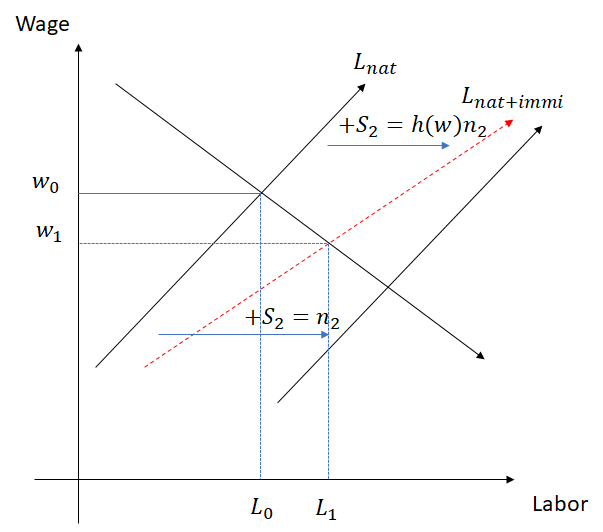
\includegraphics[width=0.55\textwidth]{Images/immigrant_effect.png}
    \caption{Effect of Immigrant supply}
    \label{fig:immigrants}
\end{figure}


\item 
By totally differentiating equilibrium conditions, derive comparative statics formulas for the elasticity of native wages and employment with respect to immigration Which economic parameters govern immigration effects? Since both type of workers have the same labor supply functions,and taking total differentiation 

\begin{equation}
\begin{aligned}
 & D(w) = n_1h(w) + n_2h(w) ;\ \text{where}  \ S_1 = n_1h(w) , S_2 = n_2h(w)  \\
 & D'(w)dw = n_1h'(w)dw + h(w)dn_1 +n_2h'(w)dw + h(w)dn_2
\end{aligned}
\end{equation}

Divide by $D(w)$ ,multiply by $\frac{w}{w}$, $\frac{n_2}{n_2}$

\begin{equation}
\begin{aligned}
 & \frac{D'(w)wdw}{D(w)w}  =  \frac{n_1h'(w)w}{S_1(w)}\frac{S_1(w)}{D(w)}\frac{dw}{w} +
 \frac{n_2h'(w)w}{S_2(w)}\frac{S_2(w)}{D(w)}\frac{dw}{w} +
 \frac{n_2h(w)}{D(w)}\frac{dn_2}{n_2} \\
 & \eta dln(w) = \epsilon_1(1-\phi)dln(w) + \epsilon_2\phi dln(w) + \phi dln(n_2)
\end{aligned}
\end{equation}


therefore the effects of immigration on wages is :

\begin{equation}
\begin{aligned}
\frac{dln(w)}{dln(n_2)} = \frac{\phi}{\eta - \epsilon_1 + \phi(\epsilon_1 - \epsilon_2)}
\end{aligned}
\end{equation}

when both types of workers have the same labor supply $\epsilon_1 = \epsilon_2$, the effects on wages will be govern positively by the immigrant share $\phi$ and the elasticity supply $\epsilon_1$ but will have a negative relation with the elasticity demand $\eta$.
It would be useful to see the effects on the employment 

\begin{equation}
\begin{aligned}
\frac{dL_1}{dn_2} = \frac{dln(S_1)}{dln(S_1)}\frac{S_1}{S_2} =   \frac{\epsilon(1-\phi) }{\eta - \epsilon_1 + \phi(\epsilon_1 - \epsilon_2)}
\end{aligned}
\end{equation}


\end{enumerate}

%\section{Question 5}
%Empirical immigration effects

\begin{enumerate}[label=(\alph*)]

\item 
Try to replicate the results in Table III of Borjas (2003) using your own Census and CPS samples from IPUMS.

\begin{table}[H]
\caption{\label{tab:table1}Impact of Immigrant Share on Labor Market Outcomes of Native Education-Experience Groups.}
\begin{center}
\def\sym#1{\ifmmode^{#1}\else\(^{#1}\)\fi} 

\begin{tabular}{lccc}
\multicolumn{4}{c}{\textit{Basic estimates}}\\
                    &\multicolumn{1}{c}{(1)}&\multicolumn{1}{c}{(2)}&\multicolumn{1}{c}{(3)}\\
\midrule
immigrant    &      -0.136&       0.021&      -0.068\\
                    &     (0.179)&     (0.129)&     (0.037)\\
\vspace{0.3mm}\\ \hline \end{tabular}         

\def\sym#1{\ifmmode^{#1}\else\(^{#1}\)\fi} 
\begin{tabular}{lccc}
\multicolumn{4}{c}{\textit{Unweighted}}\\
                    &\multicolumn{1}{c}{(1)}&\multicolumn{1}{c}{(2)}&\multicolumn{1}{c}{(3)}\\
\midrule
immigrant    &      -0.129&       0.040&      -0.080\\
                    &     (0.170)&     (0.124)&     (0.033)\\
\vspace{0.3mm}\\ \hline \end{tabular}    

\def\sym#1{\ifmmode^{#1}\else\(^{#1}\)\fi} 
\begin{tabular}{lccc}
\multicolumn{4}{c}{\textit{Includes women in labor force}}\\
                    &\multicolumn{1}{c}{(1)}&\multicolumn{1}{c}{(2)}&\multicolumn{1}{c}{(3)}\\
\midrule
immigrant    &       0.026&       0.241&      -0.084\\
                    &     (0.135)&     (0.063)&     (0.040)\\
\vspace{0.3mm}\\ \hline \end{tabular}     

\def\sym#1{\ifmmode^{#1}\else\(^{#1}\)\fi} 

\begin{tabular}{lccc}
\multicolumn{4}{c}{\textit{Includes log native labor force}}\\
                    &\multicolumn{1}{c}{(1)}&\multicolumn{1}{c}{(2)}&\multicolumn{1}{c}{(3)}\\
\midrule
immigrant    &      -0.082&       0.149&      -0.102\\
                    &     (0.266)&     (0.139)&     (0.065)\\

\vspace{0.3mm}\\ \hline  \hline \end{tabular}
\begin{tablenotes}
\begin{small}
\item
The dependent variable in (1) is Log annual earnings , Log weekly earnings in (2) and Fraction of time worked in (3). The table reports the coefficient of the immigrant share variable from regressions where variable is  the mean labor market outcome for a native education-experience group at a particular time. Standard errors are reported in parentheses and are adjusted for clustering within education-experience cells. All regressions have 160
observations and, except for those reported in row 2, are sample size of the education-experience-period cell.
\end{small}
\end{tablenotes} 

\end{center}
\end{table}

\item
Explore the robustness of your findings to the possible presence of group-specific linear trends.
\begin{table}[H]
\caption{\label{tab:table2}Impact of Immigrant Share on Labor Market Outcomes of Native Education-Experience Groups including presence of group-specific linear trends.}
\begin{center}
\def\sym#1{\ifmmode^{#1}\else\(^{#1}\)\fi} 
\begin{tabular}{lccc}
\multicolumn{4}{c}{\textit{Basic estimates}}\\
                    &\multicolumn{1}{c}{(1)}&\multicolumn{1}{c}{(2)}&\multicolumn{1}{c}{(3)}\\
\midrule
immigrant    &      -0.067&       0.167&      -0.098\\
                    &     (0.344)&     (0.241)&     (0.071)\\
\vspace{0.3mm}\\ \hline \end{tabular}        

\def\sym#1{\ifmmode^{#1}\else\(^{#1}\)\fi} 
\begin{tabular}{lccc}
\multicolumn{4}{c}{\textit{Unweighted}}\\
                    &\multicolumn{1}{c}{(1)}&\multicolumn{1}{c}{(2)}&\multicolumn{1}{c}{(3)}\\
\midrule
immigrant    &      -0.040&       0.206&      -0.113\\
                    &     (0.314)&     (0.214)&     (0.068)\\
\vspace{0.3mm}\\ \hline \end{tabular}    

\def\sym#1{\ifmmode^{#1}\else\(^{#1}\)\fi} 
\begin{tabular}{lccc}
\multicolumn{4}{c}{\textit{Includes women in labor force}}\\
                    &\multicolumn{1}{c}{(1)}&\multicolumn{1}{c}{(2)}&\multicolumn{1}{c}{(3)}\\
\midrule
immigrant    &      -0.212&       0.151&      -0.153\\
                    &     (0.218)&     (0.109)&     (0.064)\\
\vspace{0.3mm}\\ \hline \end{tabular}   

\def\sym#1{\ifmmode^{#1}\else\(^{#1}\)\fi} 
\begin{tabular}{lccc}
\multicolumn{4}{c}{\textit{Includes log native labor force}}\\
                    &\multicolumn{1}{c}{(1)}&\multicolumn{1}{c}{(2)}&\multicolumn{1}{c}{(3)}\\
\midrule
immigrant    &      -0.274&       0.090&      -0.136\\
                    &     (0.310)&     (0.158)&     (0.092)\\
\vspace{0.3mm}\\ \hline \hline \end{tabular}       

\begin{tablenotes}
\begin{small}
\item
The dependent variable in (1) is Log annual earnings , Log weekly earnings in (2) and Fraction of time worked in (3). This regressions include presence of group-specific linear trends. The table reports the coefficient of the immigrant share variable from regressions where variable is  the mean labor market outcome for a native education-experience group at a particular time. Standard errors are reported in parentheses and are adjusted for clustering within education-experience cells. All regressions have 160
observations and, except for those reported in row 2, are sample size of the education-experience-period cell.
\end{small}
\end{tablenotes} 

\end{center}
\end{table}

\end{enumerate}

%\section{Question 6}
%Human capital

\begin{enumerate}[label=(\alph*)]

\item 
Suppose that potential log earnings for a worker with s years of schooling are given by

\begin{equation}
\begin{aligned}
g_i(s) = \alpha + \rho_1s-\rho_2s^2
\end{aligned}
\end{equation}

and that potential schooling values $[S_{0i}, S_{1i}]$  indexed against a Bernoulli instrument, $Z_i$, determine
actual schooling according to

\begin{equation}
\begin{aligned}
S_i = S_{0i} + (S_{1i}-S_{0i})Z_i
\end{aligned}
\end{equation}

We need to show that the Wald estimand using $Z_i$ to instrument $S_i$ equals the average derivative $\EX[w_ig'_i(S_i^*)]$

First , the independence assumption is \{$g_i(s), S_{1i}, S_{0i}$\} $\bot Z$ , and the monotonicity assumption is $S_{1i} \geq S_{0i}$. This means the instrument is independent of what an individual could earn with schooling level S, and independent of the random elements in the first stage. Therefore the Wald estimator can be written 

\begin{equation}
\begin{aligned}
\frac{\EX[g_i(S_i)|Z_i = 1] - \EX[g_i(S_i)|Z_i = 0]}
{\EX[S_i|Z_i = 1] - \EX[S_i|Z_i = 0]} = 
\frac{\EX[g_i(S_{1i})-g_i(S_{0i})]}
{\EX[S_{1i} - S_{0i}]}
\end{aligned}
\end{equation}

Assuming that $\omega_i \equiv \frac{S_{1i} - S_{0i}}{\EX[S_{1i} - S_{0i}]}$
we can rewrite the wald stimator 

\begin{equation}
\begin{aligned}
\EX[\omega_i\frac{g_i(S_{1i})-g_i(S_{0i})}{S_{1i} - S_{0i}} ]
\end{aligned}
\end{equation}

This is a weighted average arc-slope of $g_i(S)$ on the interval $[S_{0i}, S_{1i}]$. We can simplify further using the mean value theorem where $g_i(S_{1i}) = g_i(S_{0i}) + g'_i(S_i^{*})(S_{1i} - S_{1i})$ for $S_i^{*}$ in the interval $[S_{0i}, S_{1i}]$. Therefore, we can rewrite the wald stimator as an average derivative 

\begin{equation}
\begin{aligned}
\frac{\EX[g_i(S_{1i})-g_i(S_{0i})]}
{\EX[S_{1i} - S_{0i}]} = 
\frac{\EX[(S_{1i} - S_{0i})g'_i(S_i^{*})]}
{\EX[S_{1i} - S_{0i}]} =
\EX[\omega_i g'_i(S_i^{*})]
\end{aligned}
\end{equation}

Given the monotonicity assumption , $\omega_i$ is positive for everyone.So the Wald estimator is a  weighted average of individual-specific slopes at a point in the interval $[S_{0i}, S_{1i}]$.

Now given the equation (34) let´s find the Wald estimator using the last equation , $g'_i(S_i) = \rho_1 + 2\rho_2S_i$ and $S_i^{*} = \frac{S_{1i} - S_{0i}}{2}$. 

\begin{equation}
\begin{aligned}
& g'_i(S_i^{*}) = \rho_1 + \rho_2(S_{1i} - S_{0i}) \\
& \EX[\omega_i\frac{g_i(S_{1i})-g_i(S_{0i})}{S_{1i} - S_{0i}} ] = 
\frac{\EX[(S_{1i} - S_{0i})(\rho_1 + \rho_2(S_{1i} - S_{0i}))}
{\EX[S_{1i} - S_{0i}]}
\end{aligned}
\end{equation}

Now using the normal expression of the Wald estimator 

\begin{equation}
\begin{aligned}
 \frac{\EX[g_i(S_{1i})-g_i(S_{0i})]}
{\EX[S_{1i} - S_{0i}]} 
& =\frac{\EX[\rho_1(S_{1i} - S_{0i}) - \rho_2(S_{1i}^2 - S_{0i}^2)]}{\EX[S_{1i} - S_{0i}]}  \\
& =\frac{\EX[(S_{1i} - S_{0i})(\rho_1 + \rho_2(S_{1i} - S_{0i}))]}
{\EX[S_{1i} - S_{0i}]}
\end{aligned}
\end{equation}

\item
This weighted averaging property of IV has been said to explain why IV estimates tend to exceed the corresponding OLS estimates. Lang (1993) called the IV>OLS pattern of empirical findings “discount rate bias”. Why is this pattern reasonably called “bias” and what does it have to do with discount
rates?

The expression in (39) seems to be a a weighted average of individual slopes at the midpoint of the interval $[S_{0i}, S_{1i}]$ for each person.
The fact that the weights are proportional to  $S_{1i} - S_{0i}$ sometimes has economic significance. For Lang (1993) the first-stage effect is assumed to be proportional to individual discount rates.
He propose that the natural candidate for IV could be the discount rate since is not correlated to ability. then $s = (a,r) $ , but we can invert the schooling equation to get innate ability as a function of schooling and discount rate  $i=(s,r)$. Even if innate ability and the discount rate are uncorrelated they are correlated on we condition on the level of schooling. , which means for a given level of schooling , individuals with higher discount rates have more innate ability. Then the human capital production function is $q(s,i(s,r) = q^*(s,r)$. Therefore if we regress the log wage on schooling alone, the error term contains the discount rate as one of its component. Since higher discount rates lower attained schooling, this component is correlated with education which introduces a negative bias.That is the reason why  IV>OLS.
Therefore, since people with higher discount rates get less schooling and the schooling-earnings relationship has been assumed to be concave this tends to make the Wald estimate higher than the population average return. 

\item
Card (2001) considers the evidence for discount rate bias. What does he look at? Are there alternative explanations for the pattern of empirical findings that Card describes?

He proposes that the the probability limit of the IV
estimator is 

\begin{equation}
\begin{aligned}
plim b_{iv} = \bar{\beta} + [{\sigma_{\eta}^2k_1/k + \sigma_{b\eta}(1-k_1/k)}]/\Bar{r} 
\end{aligned}
\end{equation}

If individuals with higher return to schooling have lower discount rates, then $\sigma_{b\eta}\leq0$ and the IV estimator maybe positively or negatively biased relative to $\bar{\beta}$, which represents the "discount rate bias".
He presents a table which include OLS and IV estimates of the return to education with instruments based on features of the school system from 1991 to 1999. This table shows that IV  estimates return to schooling typically exceed the corresponding OLS estimates, often by 20 percent or more. Since OLS lead to upward-biased estimates of the true causal effect, the even larger IV present an issue that needs to be explained. 
There are some other explanations for this puzzle. First, ability biases in the OLS estimates of the return to schooling are relative small and the gap between IV-OLS reflect downward bias in the OLS estimates attributable to measurement errors. 
Second, IV are even further upward biased than OLS by unobserved differences between the characteristics of the treatment and comparison groups implicit in the IV scheme. 
Third, the "specification searching" in comparing alternative IV specifications , researchers tend to favor those that yield a higher t statistic for the estimated return to schooling. 
Finally, there is underlying heterogeneity in the returns to education and that many of the IV estimates based on supply-side innovations tend to recover returns to education for a subset of individuals with relatively high return to education. 


\end{enumerate}

\end{document}
